\documentclass[a4paper,twoside]{article}
\usepackage{algorithm}
\usepackage{algpseudocode} 
\usepackage[babel,german=quotes,english=american]{csquotes} 
\usepackage[pdftex]{graphicx}
\usepackage{url}
\usepackage{pgfplots}

\usepackage{epsfig}
\usepackage{subcaption}
\usepackage{calc}
\usepackage{amssymb}
\usepackage{amstext}
\usepackage{amsmath}
\usepackage{amsthm}
\usepackage{multicol}
\usepackage{pslatex}
\usepackage{apalike}
\usepackage{SCITEPRESS}     % Please add other packages that you may need BEFORE the SCITEPRESS.sty package.

%\subfigtopskip=0pt
%\subfigcapskip=0pt
%\subfigbottomskip=0pt

\begin{document}

\title{Probabilistic Symbol Encoding for \\Convolutional Associative Memories}

\author{\authorname{Igor Peric, Alexandru Lesi, Daniel Spies, Stefan Ulbrich,\\ Arne R{\"o}nnau, Marius Z{\"o}llner and R{\"u}diger Dillman}
\affiliation{FZI Forschungszentrum Informatik, Karlsruhe, Germany}
\email{\{peric, lesi, spies, ulbrich, roennau, zoellner, dillmann\}@fzi.de}
}

\keywords{Vector Symbolic Architectures, Associative Memories, Symbol Encoding, Symbolic Scripting}

\abstract{		Vector Symbolic Architectures (VSAs) define a set of operations
		for association, storage, manipulation and retrieval
		of symbolic concepts, represented as fixed-length vectors in
		${\rm I\!R}^n$.
		A specific instance of VSAs, Holographic Reduced Representations (HRRs),
		have proven to exhibit properties similar to human short-term
		memory and as such are interesting for computational modelling.
		In this paper we extend the HRR approach by introducing implicit,
		topology-preserving encoding and decoding procedures.
		We propose to replace unique symbolic representations with symbols based on
		probability density functions.
		These symbols must be randomly permuted to ensure the uniform distribution of signals across Fourier space where
		embedding takes place.
		These novel encoding schemes eliminate the need for so-called \emph{clean-up modules} after memory
		retrieval (e.g., self-organizing maps). Effectively each encoding
		implicitly represents its scalar symbol, so no further lookup is needed.
		We further show that our encoding scheme has a positive impact
		on memory capacity in comparison to the original capacity
		benchmark for HRRs \cite{Plate:1995:HolographicReducedRepresentations}.
		We also evaluate our memories in two different robotics tasks: visual scene memory and state machine scripting (holographic controllers).}

\onecolumn \maketitle \normalsize \vfill

	\section{INTRODUCTION}
	
	Vector Symbolic Architectures (VSA) define a set of operations for storage (compression) and retrieval of symbolic concepts in fixed size vectors.
As described in \cite{Levy:2008:VectorSymbolicArchitectures}, every VSA has to implement three basic operations:
	\begin{enumerate}
		\item association (binding) $\mapsto \otimes$
		\item superposition (appending) $\mapsto +$
		\item probing (unbinding) $\mapsto \oslash$
	\end{enumerate}
	
	VSAs can be viewed as a lossy compression technique, since binary operations on N-element vectors return N-element vectors as well. These operations will be described in further detail in the following section. 
	
	\begin{figure}
		\center
		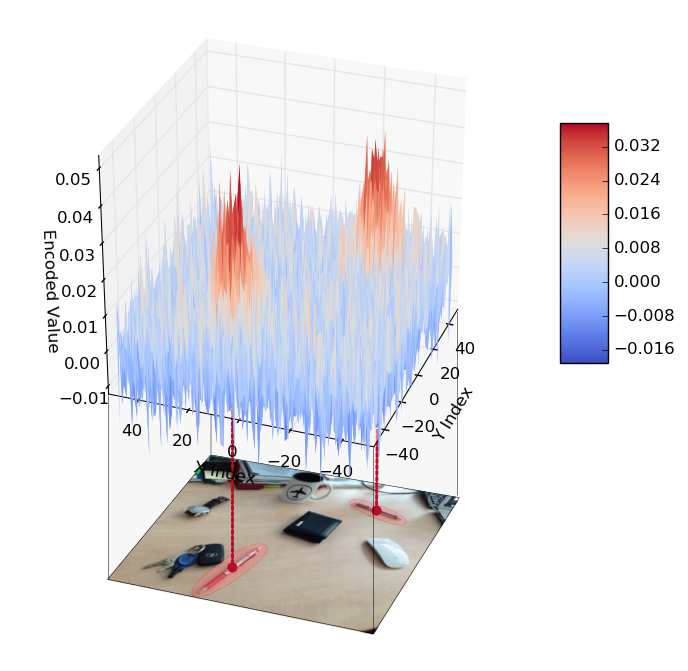
\includegraphics[width=0.9\columnwidth]{img/probe_for_pen_w_img.png}
		\caption{In-memory probability for a symbol "pen"}
	\end{figure}	
	
	Depending on the way these three operations are implemented we can distinguish several popular VSAs, such as Holographic Reduced Representations \cite{Plate:1995:HolographicReducedRepresentations}, Circular HRRs \cite{DeVine:2010:Semanticoscillations}, Binary Spatter Codes \cite{Kanerva:1994:SpatterCodeEncoding}, Holographic Graph Neurons \cite{Kleyko:2016:HolographicGraphNeuron}, Geometric Algebras \cite{Patyk-Lonska:2011:DistributedRepresentationsBased} and Random Permutations \cite{Recchia:2015:EncodingSequentialInformation}.
The most widely used ones are HRRs and they are briefly explained in section \ref{sec:hrr}.
Authors in \cite{Golosio:2015:CognitiveNeuralArchitecture} have used them to solve word embedding problems for extremely large datasets by replacing computationally expensive big matrix factorizations with an iterative estimation algorithm.
Some of the other work is centered around pattern recognition \cite{Kleyko:2016:PatternRecognitionVector} and functional large-scale cognitive architecture models \cite{Eliasmith:2012:LargeScaleModel}.
Preliminary theoretical assumptions have been made about the ability to use them as agent controllers \cite{Levy:2013:LearningBehaviorHierarchies}, where a symbolic program is represented with a set of combined symbolic actions associated with actuator symbols and symbolic sensing.
		
	Authors in \cite{Eliasmith:2012:LargeScaleModel} have demonstrated that the functional cognitive model Spaun is capable of performing $7$ different cognitive tasks when implemented as HRRs using biologically plausible models of neuron dynamics.
They further show that in serial working memory tasks the model of forgetting exhibits similar behaviour as human working memory due to limited capacity.
Lastly they report similarity between the human working memory capacity and the average number of items (symbols) that their model is capable of holding in memory.

	This successful model of forgetting is one of the reasons our work is centred around HRRs. Another reason is the fact that HRRs are the only VSAs up to date operating on convolution operations in their core.
This is appealing if we take the numerous recent advancement in deep learning and convolutional neural networks into consideration.
These networks succeed due to training on big data and using convolution as the main architectural constraint.
Although the description of the biophysical mechanism underlying convolution and the concept of weight sharing are still missing, it is important to reuse proven concepts, such as convolutional filtering, in a way as general as possible.
In other words, addressing multiple fundamentally different problems with similar computational principles can be considered a step towards a unified brain processing theory.
	
	\section{VECTOR SYMBOLIC ARCHITECTURES}
	
In order to use VSA operations all types of required inputs need to first be represented as symbols, which are vectors of fixed size. The basic approach is to pick these vectors randomly once for each input used in any operation and maintain these pairs in a separate data structure.	
	\\
	
	\textbf{Association} (also called "binding") is the operation of linking two operands together, resulting in a vector of the same size which is dissimilar (or orthogonal) to the original vectors, but also contains scrambled information from both of them.
For instance, linking the property "red" to object "triangle" can be done using the binding operation as follows:
	
	\begin{equation}
	memory_1 = red \otimes triangle
	\end{equation}
	
	\textbf{Superposition} is the operation of extending a symbol, regardless of what it already contains.
The memory "red triangle and blue circle" is formed as:
	\begin{equation}
	memory_2 = memory_1 + blue \otimes circle
	\end{equation}
	
	\textbf{Probing} is the operation of extracting a noisy version of an associated item from a set memory.
Asking "What color is the triangle?" works as follows:
	
	\begin{equation}
	red \approx memory_2 \oslash triangle
	\end{equation}
	
	
	The probing operation assumes the existence of inverse elements, so the previous equation can be interpreted and explained as such:
	\begin{multline}
	memory_2 \otimes triangle'=\\
	(red \otimes triangle + blue \otimes circle) \otimes triangle'=\\
	red \otimes triangle  \otimes triangle' + blue \otimes circle \otimes triangle' =\\
	red + blue \otimes circle \otimes triangle'  = red + noise
	\approx red
	\end{multline}
	
	Here $triangle'$ represents the inverse of $triangle$.
The resulting vector will be a composition of something that is very similar to $red$ and something that doesn't resemble anything meaningful from the symbol table, so it can be treated as negligible noise. One similarity measure is the cosine distance, which for two vectors \pmb x and \pmb y is calculated as follows:
	
	\begin{equation}
cos(\pmb x, \pmb y) = \frac {\pmb x \cdot \pmb y}{||\pmb x|| \cdot ||\pmb y||}
	\end{equation} 
	
	Obtained similarity values clearly distinguish the matching vectors. Concrete values that highlight this will be later presented in section \ref{sec:experiments}.	

	The process of converting the noisy result of probing into the closest known symbol is called the \textbf{clean-up procedure}.
A straightforward way of implementing clean-up memory is using a lookup table, while other researchers show that any type of attractor network can be used (e.g. self-organizing maps).

	In the case of lookup tables, in order to decode a specific symbolic vector, the elements from a symbol table are iterated over, the similarity to each of the entries is calculated and the symbol which presented maximum similarity is returned. With the help of a threshold for the similarity value false-positives can be excluded. A lookup requires $O(n)$, where $n$ is the number of symbols known to the system. This approach works quite well for object identifiers (names), but has some non-desirable properties when used on scalar encoding. The space complexity will increase and may become infeasible, depending on the number of inputs needed. One way of handling symbolic scalar encoding is to discretize the whole input range into bins and assigning a random vector to each discrete value. This, however may often prove to not satisfy the task needs any more.
In this paper, we present an intrinsic, probabilistic encoding and decoding
method, which removes the necessity of using a symbol table.

	\subsection{Holographic Reduced Representations}
	\label{sec:hrr}
	
	Holographic Reduced Representations are VSAs which implement the operation of binding as circular convolution. One option for calculating it is with the help of discrete Fast Fourier Transformations (FFTs). Taking $f(x)$ to describe an FFT, with its inverse $f^{-1}(x)$, circular convolution is calculated as:
	
	\begin{equation}
	\pmb a = f^{-1}(f(\pmb x) * f(\pmb y))
	\end{equation}
	
	Here $\pmb a$ is the result of convolution, and $\pmb x$ and $\pmb y$ are symbolic vectors of size $n$.
Superposition is implemented as a simple element-wise vector addition. Taking the previous result and superposing it with some vector $\pmb b$ is done as follows:

	\begin{equation}
	\pmb m = \pmb a + \pmb b
	\end{equation}

The resulting vector of the superposition operation $\pmb m$ can then be probed
by using the inverse of circular convolution, which is circular correlation.
Probing can be viewed as binding with the "inverse":
	
	\begin{equation}
	\pmb y^* = f^{-1}(f(\pmb m) * f(\pmb x)^{-1})
	\end{equation} 

Following this series of operations the vector $\pmb y^*$ will be similar to vector $\pmb y$, but not entirely the same due to the noisy influence of $\pmb b$. The inverse in Fourier space referred to here is gained by calculating the complex conjugate of the vector's entries, which is done by negating the imaginary parts.
		
	Performing FFTs has no invariant regarding the mean of the resulting vector entries and can produce all sorts of results.
Due to this, when probing, we would receive vectors which had the correct relative distance between their values, i.e.
the correct "shape", but would be shifted, stretched or squeezed along the Y-axis. This lead to vectors falsely being regarded as dissimilar to each other, and can be solved by performing two normalization steps before comparing:

	\begin{equation}\label{eq:norm1}
		{x_i}' = x_i - \frac{\sum_j x_j}{|{\pmb x}|}\qquad {\pmb x}{'}{'} = \frac{{\pmb x}'}{ \| {\pmb x}'\|}
	\end{equation}
	
	\section{TOPOLOGY-PRESERVING ENCODING}
	
	\subsection{Encoding Scalar Symbols}
	
	Encoding scalars is a good example for the necessity of preserving topology.
Depending on what dataset is in use it may be required to store mappings for any number of values, which can drastically increase space requirements.
Furthermore, using a separate random encoding for each scalar, regardless of whether they are very close to each other or not, there would be no similarity in neighbouring values.
For example, the following probe will yield no result:
	
	\begin{equation}
	(10000 \otimes a) \oslash 10001
	\end{equation}
	
	To facilitate these two qualities scalar encoding can be achieved using probabilistic instead of exact symbolic representation. 
The encoded vector can simply be a Gaussian shaped probability distribution sampled over a fixed input range, with a mean equal to the encoded value and arbitrarily chosen standard deviation.
Figure \ref{no-perm-a} shows how such an encoded vector looks like, and what the result of binding it to a generic random vector is.
With this result it becomes obvious that unfortunately lots of information is lost.
If this result is probed with the symbol for "ball" something similar to the initial Gaussian distribution for the value $8$ on a scale to $10$ is expected.
And yet figure \ref{no-perm-b} presents no such outcome.
While there is a peak at the initial value lots of other peaks also arise, making it impossible to detect which one is correct.

	
	\begin{figure}[th!]
		\begin{subfigure}{1\columnwidth}
			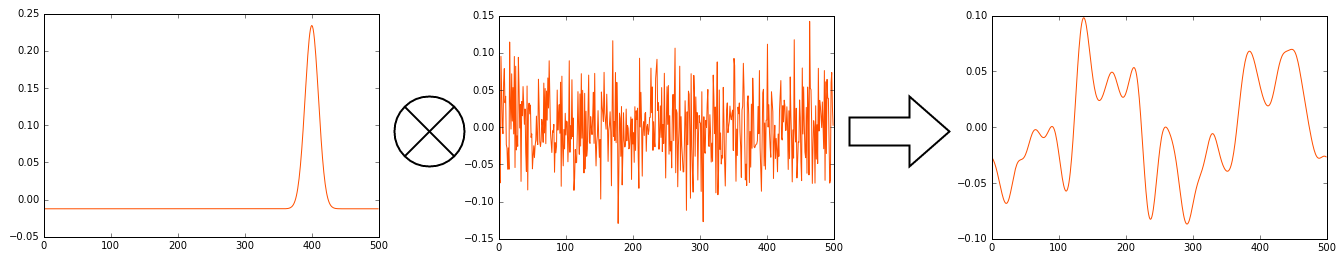
\includegraphics[width=\columnwidth]{img/scalar-pre-perm.png}
			\caption{Binding}
			\label{no-perm-a}
		\end{subfigure}
		\begin{subfigure}{1\columnwidth}
			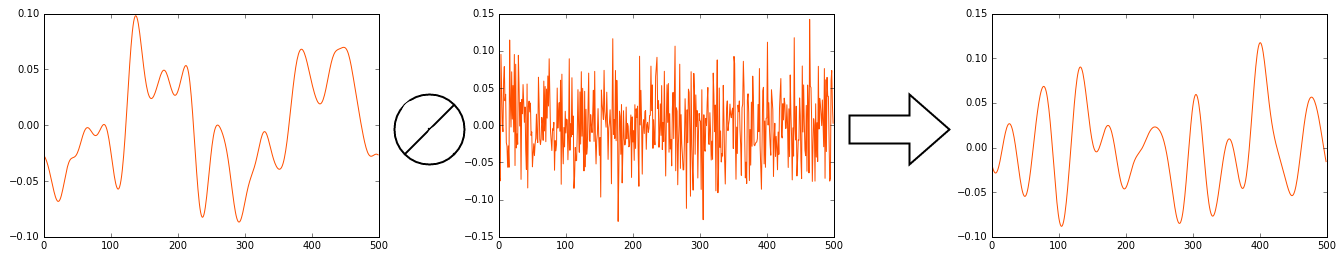
\includegraphics[width=\columnwidth]{img/scalar-pre-perm-probe.png}
			\caption{Probing}
			\label{no-perm-b}
		\end{subfigure}
		\caption{Binding 8 with "ball", then probing for "ball"}
		\label{no-perm}
	\end{figure}
	
	This effect is due to the fact that circular convolution is based on Fourier transformations. A lack of frequencies in the Fourier space of the encoded scalar becomes apparent, as highlighted in figure \ref{fft}.
All the information of a Gaussian distribution is crammed into the lowest and highest values of the Fourier transformation, resulting in a high loss of information.
In these circumstances, when probing for a scalar, the vector received is in turn recreated of too few frequencies and will not come close to resembling the original Gaussian distribution.


\begin{figure}[th!]
	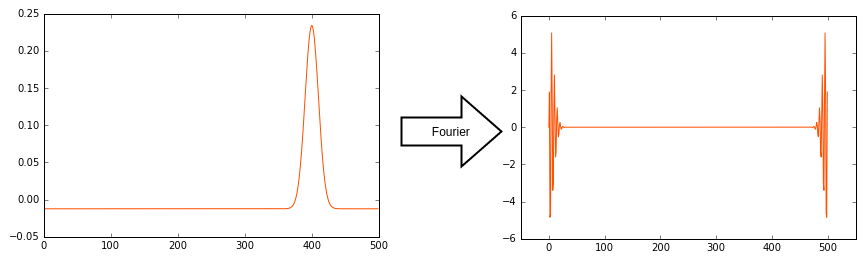
\includegraphics[width=\columnwidth]{img/scalar-pre-perm-fft.png}
	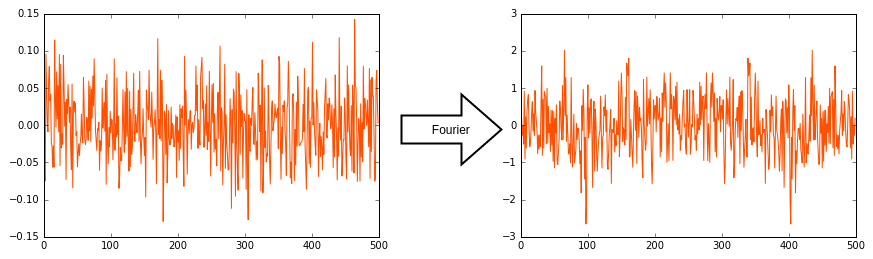
\includegraphics[width=\columnwidth]{img/scalar-random-fft.png}
	\caption{Fourier analysis of scalars and random symbols}
	\label{fft}
\end{figure}
	
	This inconvenience is removed with the help of permutations.
Depending on the size of the memory vectors used a fixed permutation is generated once.
Whenever a scalar is encoded the Gaussian distribution is first sampled over the given range, after which the sampled values swap places accordingly.
As such the resulting vector will present lots of jumps in value, which have a significant impact on the Fourier space, as can be seen in figure \ref{perm-fft}. Decoding scalar values will require a reverse permutations of the result of probing.
	
	\begin{figure}
		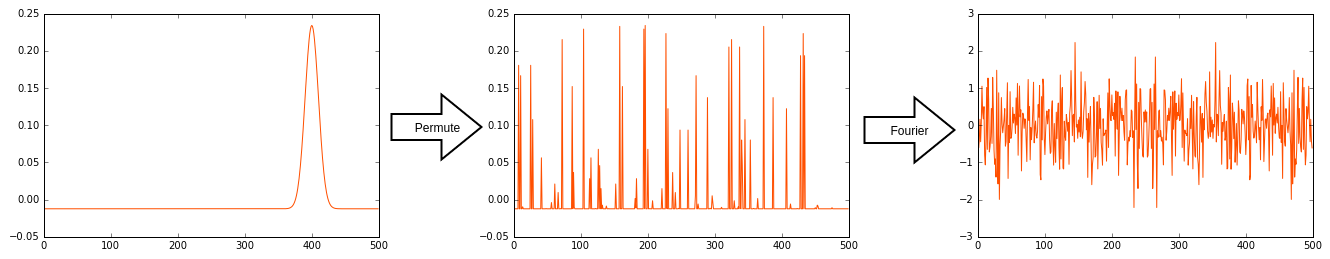
\includegraphics[width=\columnwidth]{img/scalar-perm-step-fft.png}
		\caption{Fourier space of a permuted scalar encoding}
		\label{perm-fft}
	\end{figure}
	
	Working with such a vector makes it possible to successfully probe for scalars and receive a Gaussian distribution overlapped with some noise.
All of this can be seen in figure \ref{perm}, which depicts the exact same operations as figure \ref{no-perm}, but using a permuted version of a Gaussian distribution.
The result in figure \ref{perm-b} clearly shows a spike at the expected spot in the sample range.
This vector can now be smoothed out, after which the peak can easily be identified and the initial scalar can be recovered.
	
	\begin{figure}
		\begin{subfigure}{1\columnwidth}
			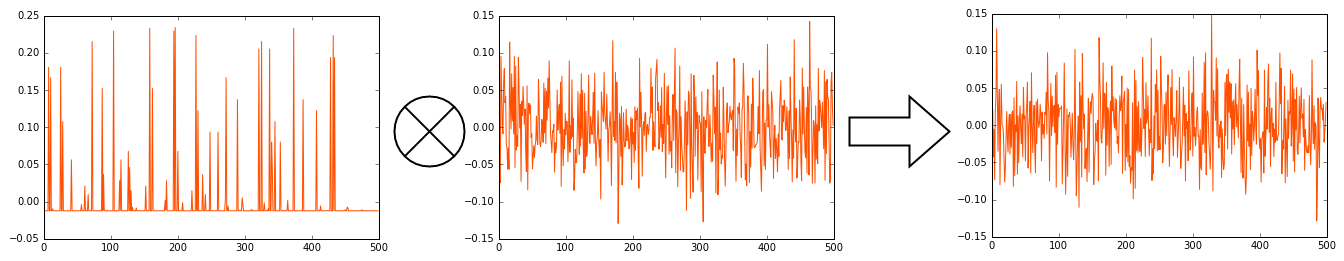
\includegraphics[width=\columnwidth]{img/scalar-post-perm.png}
			\caption{Binding}
			\label{perm-a}
		\end{subfigure}
		\begin{subfigure}{1\columnwidth}
			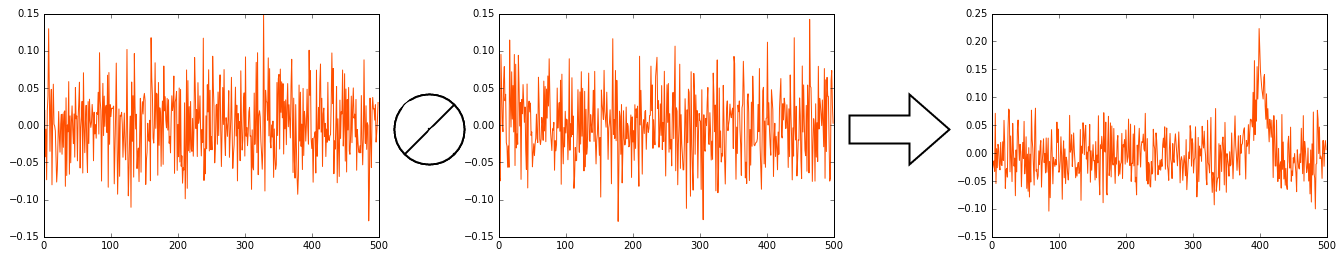
\includegraphics[width=\columnwidth]{img/scalar-post-perm-probe.png}
			\caption{Probing}
			\label{perm-b}
		\end{subfigure}
		\caption{Operations of figure \ref{no-perm} with permutation}
		\label{perm}
	\end{figure}
	
		As such using the scalar encoder simplifies the operations pipeline of working with symbols. Encoding the same scalar over and over will always yield the same result, removing the need to store scalar symbols in a lookup table. Also, when probing for a scalar, the symbol doesn't need to be matched against all other known symbols to determine the highest similarity, which can be computationally expensive. Instead the result of probing is smoothed out and verified for the presence of a Gaussian distribution, which then determines the scalar it represents. 
		

	\subsection{Encoding Coordinate Symbols}
			
		Encoding coordinate symbols works in a manner very similar to encoding scalar symbols. Depending on the number of coordinates the symbolic vectors shape is reinterpreted. 2D coordinates, for instance, require a matrix. This matrix represents the entire coordinate space and on it 2D Gaussian distributions are sampled. It can be viewed as a heat map, as displayed in figure \ref{fig:encoding-coord}.	The matrix will still be treated as a vector when it comes to running operations on it and must also be permuted. Since the value space now has more dimensions the size of the vector has to be raised accordingly to achieve performance similar to that of scalar symbol encoding. 
		
		An attempt has been made to overcome the curse of dimensionality by splitting the vector up in the number of dimensions and simply encoding the value for each dimension in the resulting sub-vectors. Unfortunately it then becomes impossible to differentiate among multiple coordinates encoded in the same vector. Specifically, when decoding, there is no way to know which of the values in separate sub-vectors belong to each other and which don't. On the other hand if only a single coordinate needs to be bound to another symbol this approach is still feasible and will permit the use of smaller vectors for high accuracy. Concretely, for $d$ dimensions, splitting up the vector will require the size to be raised by a factor of $d$ to maintain the same accuracy. Reinterpreting the shape will require the size to increase exponentially by the power of $d$ to keep the accuracy.
			
	\section{PROPERTIES OF HOLOGRAPHIC MEMORIES}
	
	Vector Symbolic Architectures in general have the following properties:
	\begin{itemize}
		\item The number of items stored in a single memory vector is not known based solely on it's content.
		\item Existence of an item in memory cannot be checked explicitly. The closest equivalent is to probe the memory for the item of interest and to compare the similarity of the decoded result to anything meaningful. Even then it could be that the result of probing for anything might still require to be probed by a further symbol to retrieve the sought out item.
		\item Chances of successful recall depend on the actual stored data.
		\item Memories can be changed in an online fashion. There is no need to recreate memories from scratch - symbols can be appended to or removed from already existing memory vectors if present.
	\end{itemize}
	
		\begin{figure}[th!]
			\begin{subfigure}{0.45\columnwidth}
				\center
				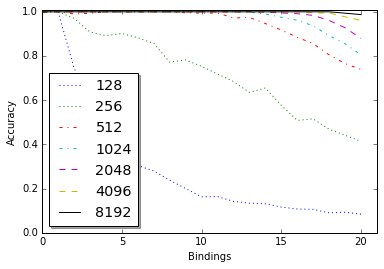
\includegraphics[width=1\columnwidth]{img/capacity.png}
				\caption{Symbols accuracy}
				\label{fig:capacity}
			\end{subfigure}
			\begin{subfigure}{0.45\columnwidth}
				\center
				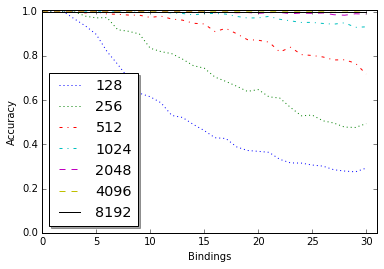
\includegraphics[width=1\columnwidth]{img/capacity_scalar_30.png}
				\caption{Scalars accuracy}
				\label{fig:capacity_scalar}
			\end{subfigure}	
			\center
			\begin{subfigure}{0.45\columnwidth}
				\center
				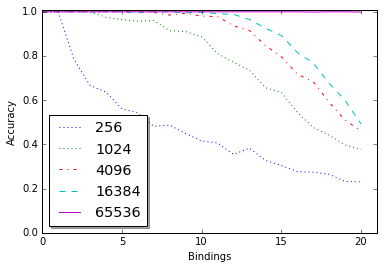
\includegraphics[width=1\columnwidth]{img/capacity_coordinate.png}
				\caption{Coordinates accuracy}
				\label{fig:capacity_coordinate}
			\end{subfigure}	
			\caption{Single vector memory capacity analysis}
		\end{figure}	
	
	
	\subsection{Capacity}
	
	Just as Plate has done in the original HRR paper \cite{Plate:1995:HolographicReducedRepresentations} we have tested the memory capacity in terms of accuracy of successful recall for variable numbers of bound pairs. Results are shown in figure \ref{fig:capacity}.
	
	As we can see, a $512$ element vector starts decreasing accuracy of recall after $10$ pairs stored in a single memory block. A $4096$ and $8192$ element vectors can almost perfectly recall $20$ associated pairs, which matches the results of Plate using a lookup table and a clean-up process. 
	
	The experiment was repeated for superposing bounded pairs of a random symbol and a scalar, as well as pairs of a random symbol and a 2D coordinate. Figure \ref{fig:capacity_scalar} shows the result for scalars. In this instance the probe was always done for the scalar value. The total accuracy of the result depends on new factors, the main of which will be the quality of the smoothing function used to clean up the noise from the resulting signal. This will determine how much the peaks position may shift in some direction. In our experiments a Hanning window smoothing technique was used and a $2\%$ deviance from the exact initial scalar was allowed. With these settings probing performed significantly better than solely among random symbols. Vectors of size 8192 even managed to maintain $100\%$ accuracy when storing $30$ bindings. Intuitively this can be explained as follows: Gaussian distributions are far more noise tolerant than random vectors. Vectors need to maintain a high similarity to be declared identical, whereas Gaussian distributions only need to present peaks after smoothing. 
	
	Finally figure \ref{fig:capacity_coordinate} shows the accuracy of stacking bindings of 2D coordinates with random symbols. The same smoothing and deviance settings were used as for the previous experiment. As coordinates are encoded in a vector that is virtually cast to 2D its length would have to be squared to achieve similar performance to scalars. Due to this higher steps in between vector lengths have been used, and most lengths still perform rather poorly. However, increasing the length considerably, like in the case with $65536$ elements, near-perfect accuracy can still be upheld up to $20$ bindings. In all $3$ experiments both fakse positives and false negatives are regarded.
		

		
	\section{EXPERIMENTS}
	\label{sec:experiments}
	\subsection{Visual Short Term Memory and Top-Down Attention Model}
	
	In this experiment a system is given a monocular stream as an input. An arbitrary algorithm is used to perform object detection and recognition, resulting in a number of 2D coordinates associated with respective object names (figure \ref{fig:object-detection}). Object names are strings and are encoded as random vectors of length $n$ (figure \ref{fig:encoding-object}). The locations of objects in the image plane are 2D coordinates $(x,y)$ and they are perceptually grounded symbols (figure \ref{fig:encoding-coord}, non-permuted).

	
	\begin{figure}[th!]
		\center
		\begin{subfigure}{1.0\columnwidth}
			\center
			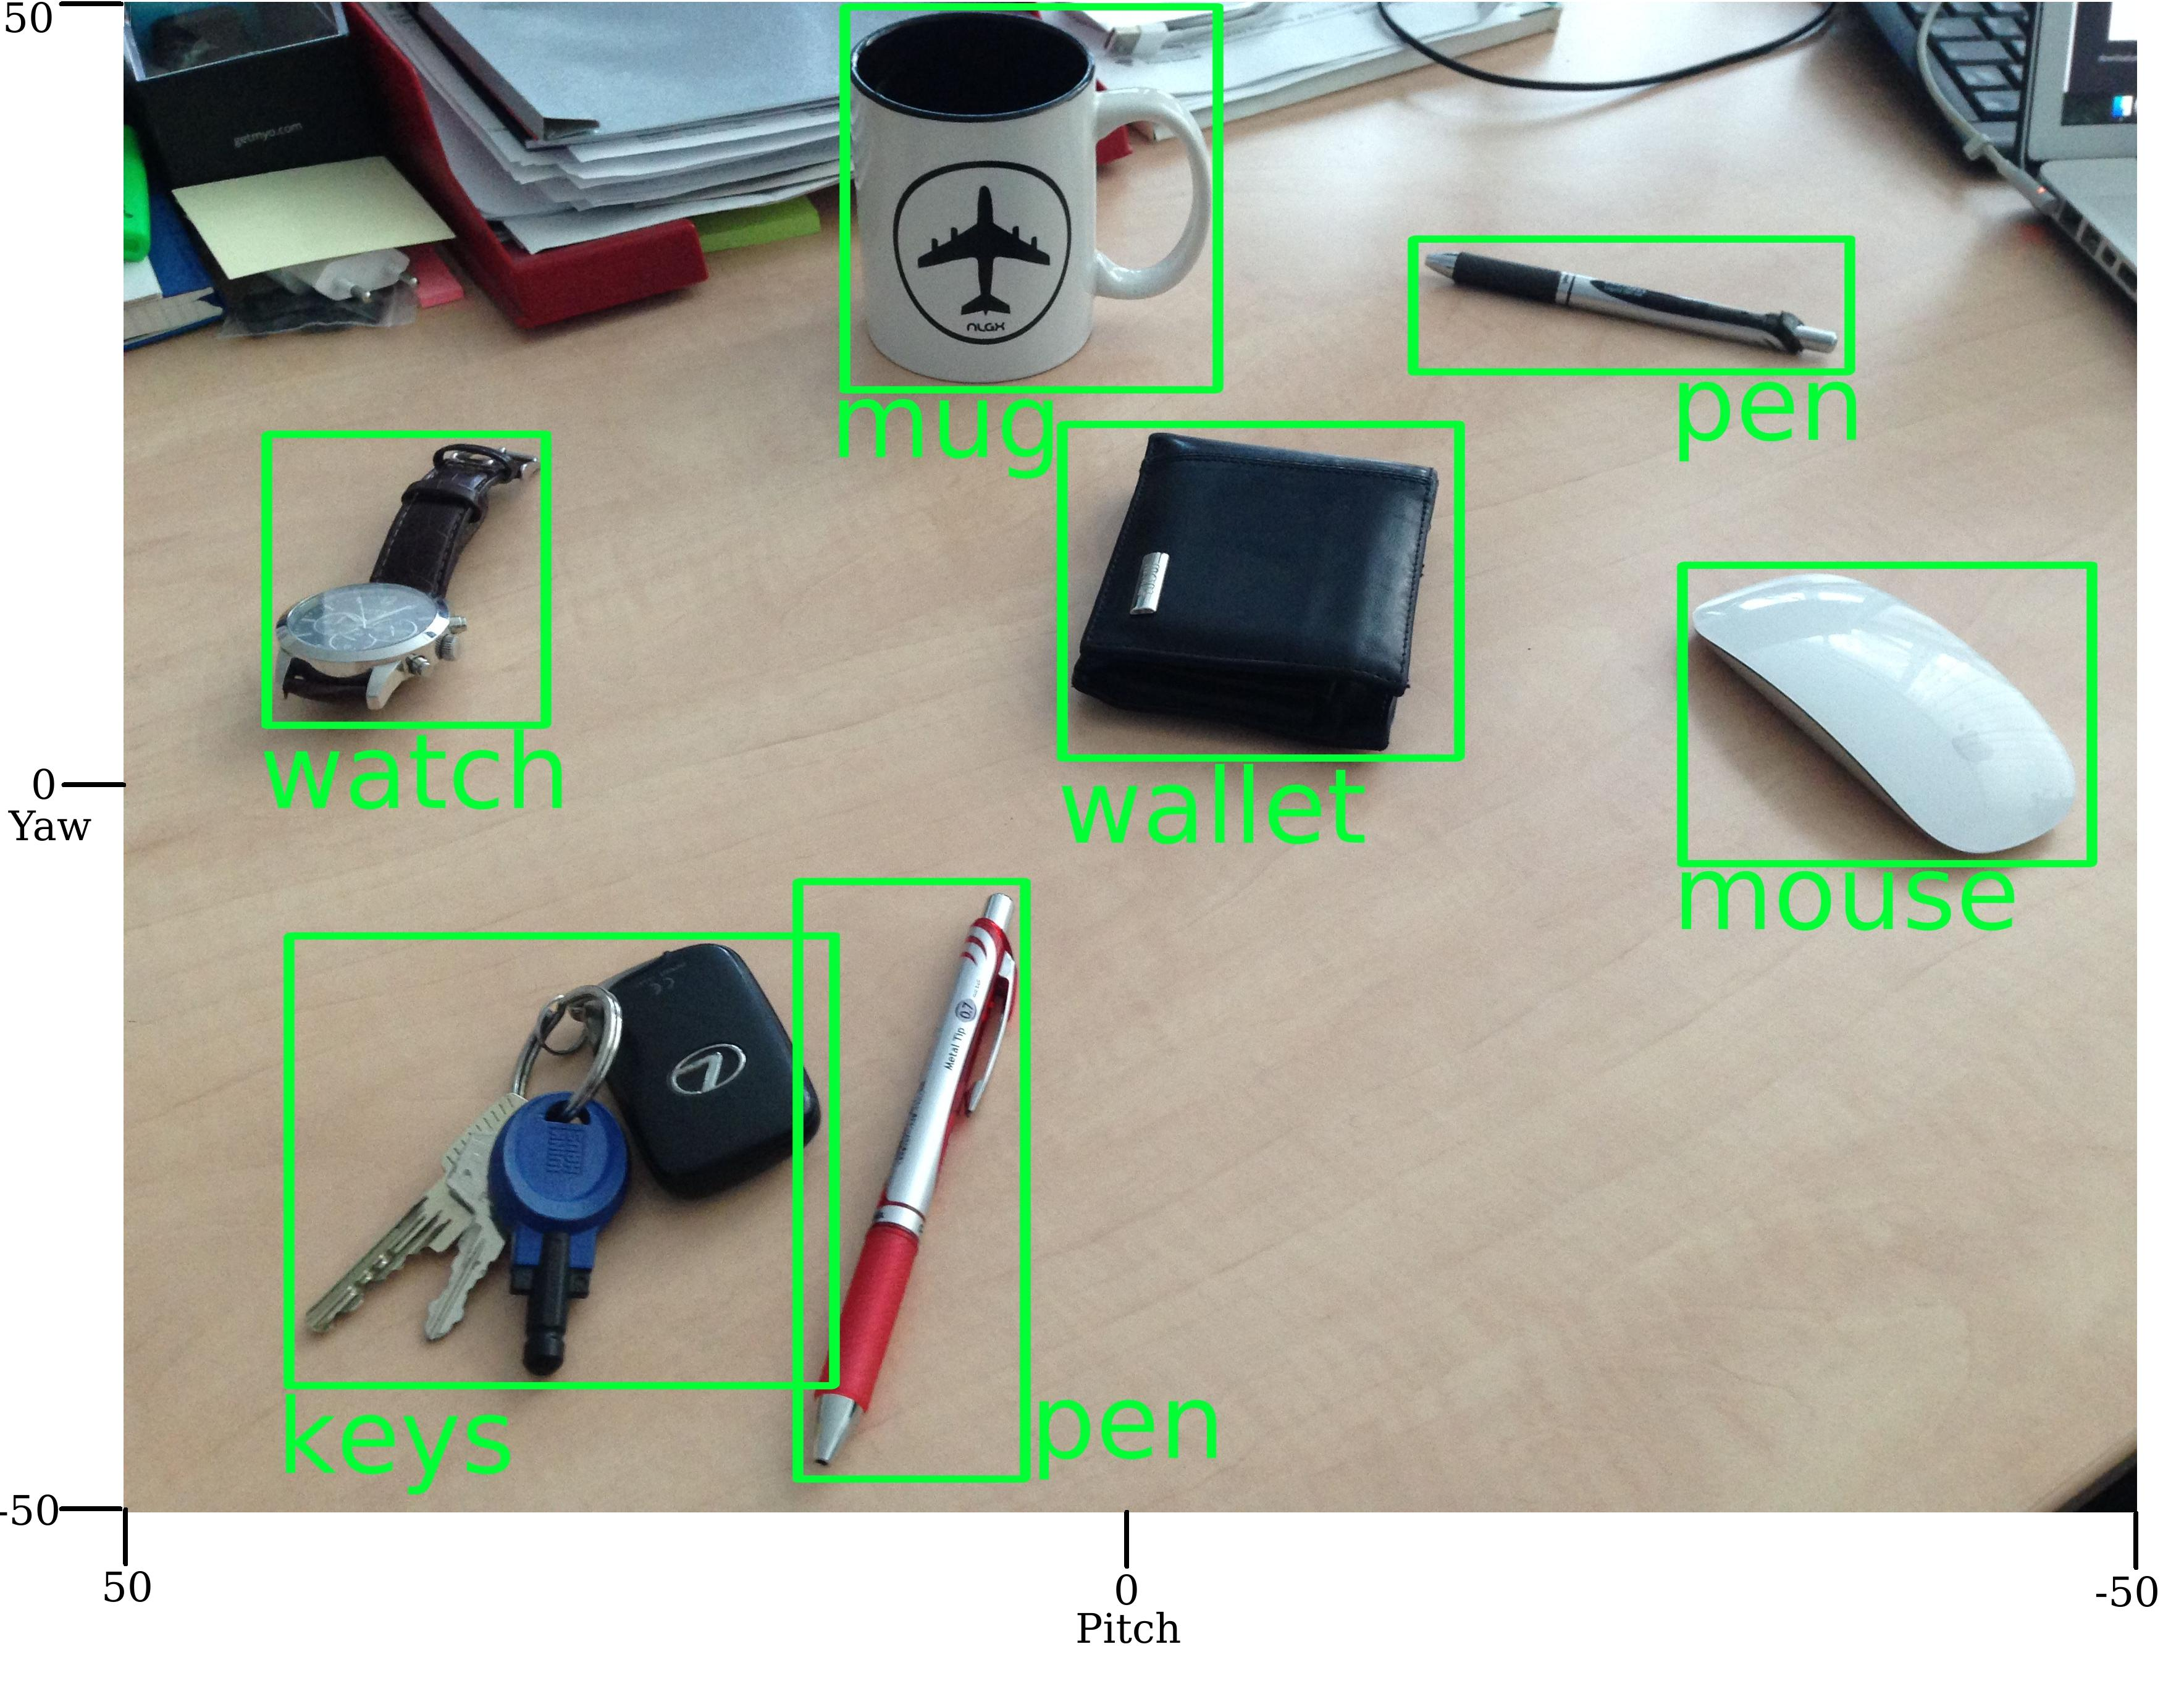
\includegraphics[width=0.6\columnwidth]{img/map_ticks.jpg}
			\caption{Original scene and a set of detected objects}
			\label{fig:object-detection}
		\end{subfigure}
		
		\begin{subfigure}{0.45\columnwidth}
			\center
			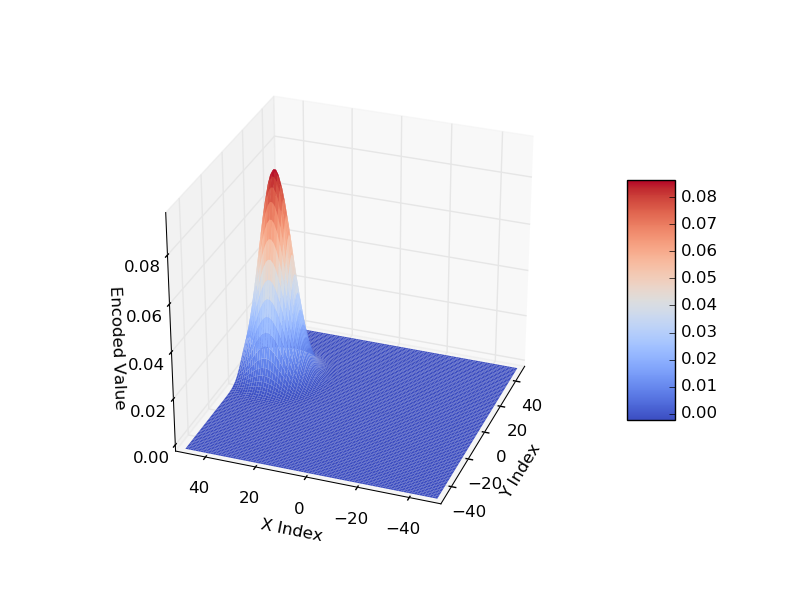
\includegraphics[width=\linewidth]{img/coord_example_1.png}
			\caption{Location of "watch"}
			\label{fig:encoding-coord}
		\end{subfigure}
		\begin{subfigure}{0.45\columnwidth}
			\center
			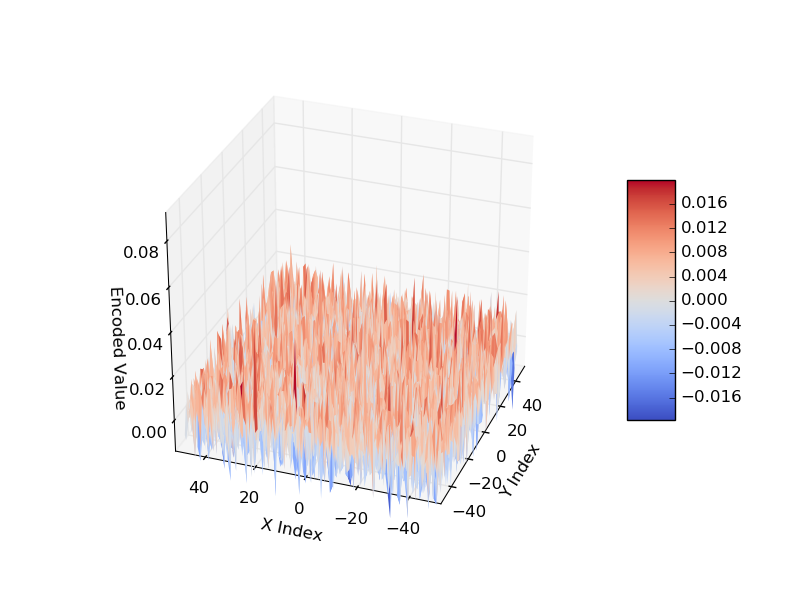
\includegraphics[width=\linewidth]{img/coord_example_2.png}
			\caption{Symbol of "watch"}
			\label{fig:encoding-object}
		\end{subfigure}
		
		\begin{subfigure}{0.8\columnwidth}
			\center
			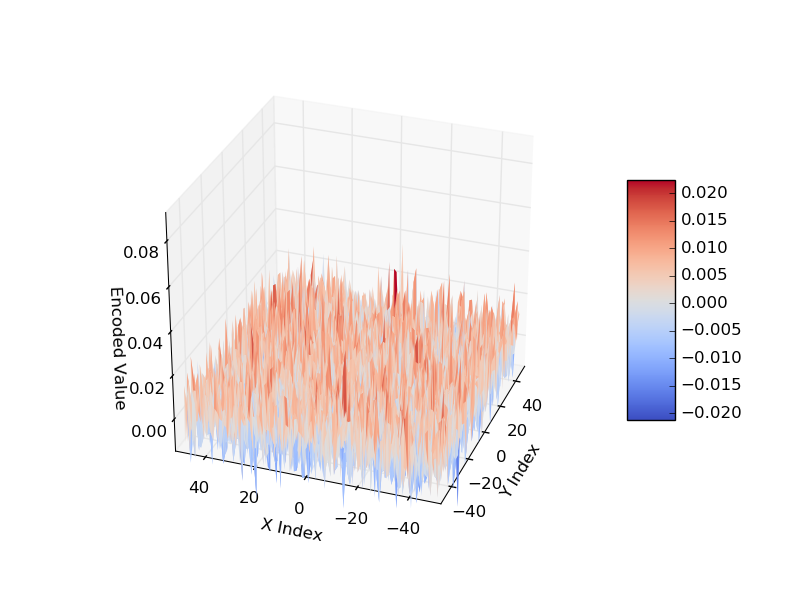
\includegraphics[width=0.8\linewidth]{img/coord_example_3.png}
			\caption{Entire  visual scene memory (7 pairs)}
			\label{fig:encoding-scene}
		\end{subfigure}
		
		\begin{subfigure}{0.45\columnwidth}
			\center
			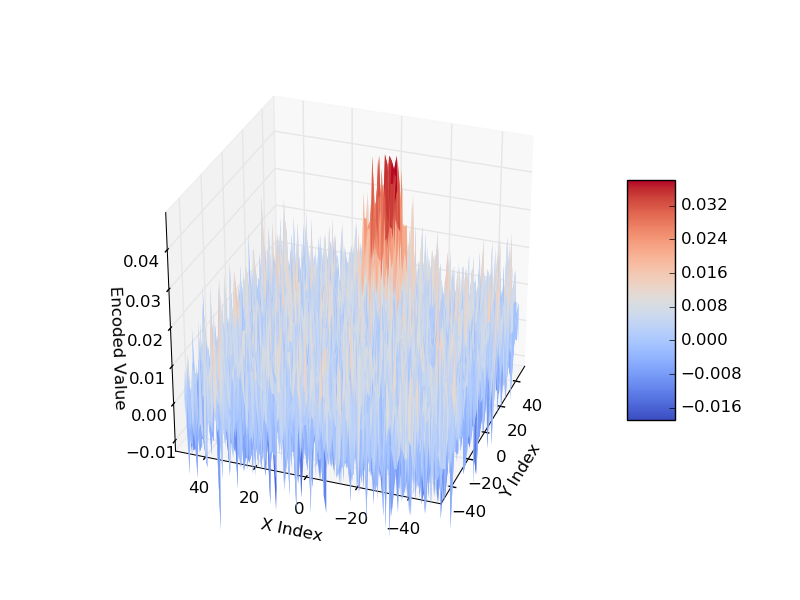
\includegraphics[width=\linewidth]{img/probe_for_mug.png}
			\caption{Probing for "mug"}
			\label{fig:probing-single}
		\end{subfigure}
		\begin{subfigure}{0.45\columnwidth}
			\center
			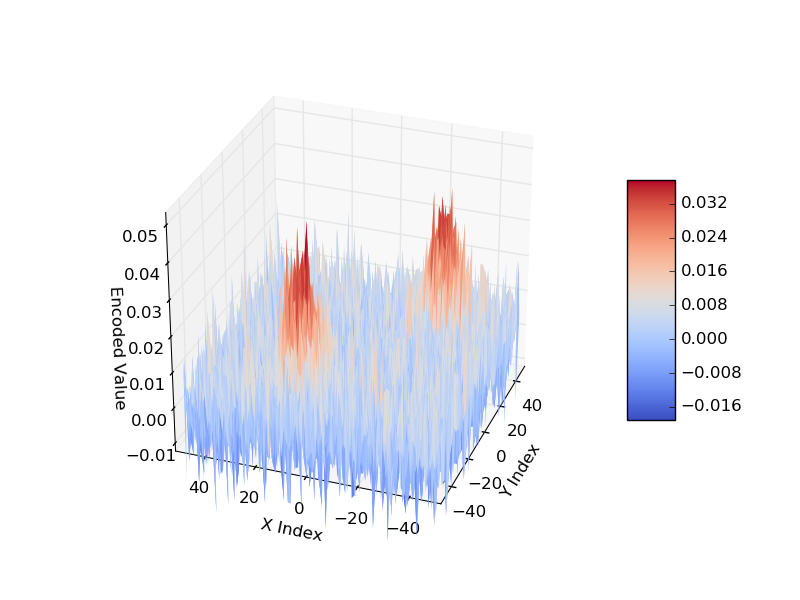
\includegraphics[width=\linewidth]{img/probe_for_pen.png}
			\caption{Probing for "pen"}
			\label{fig:probing-double}
		\end{subfigure}
		
		\caption{Representation of visual scene in memory. }
		
	\end{figure}
	
	Due to the noisy nature of probing given by the slight loss of information in the binding process each symbol may have some amount of similarity to whatever other symbol it is compared to. However, even though this is the case, the similarity measure of bound symbols is consistently higher and can be clearly distinguished from others. Chart \ref{pgf:bar1} represents the result of probing at $(19, -26.75)$, which is somewhere in between the keys and the red pen, as seen in figure \ref{fig:object-detection}.
	
	 As we can see all symbols that are nowhere near the position present similarities well below $0.05$ (values may also be negative), while both close matches scored over $0.2$. Spot on probes may even attain values of over $0.5$. The example in chart \ref{pgf:bar2} is for a probe at $(-13, 21.5)$, which is further away from the center of an object region. But even though the dark pen and the wallet are further apart the result of probing still yields distinctly higher similarities for them as opposed to objects further away. 
	
	\begin{figure}[th!]
	\center
		\begin{subfigure}{0.49\columnwidth}
	    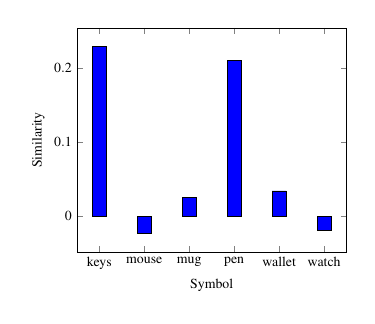
\begin{tikzpicture}[yscale=0.5, xscale=0.5]
        \begin{axis}[
            symbolic x coords={keys, mouse, mug, pen, wallet, watch},
            xlabel = Symbol,
            ylabel = Similarity
          ]
            \addplot[ybar,fill=blue] coordinates {
                (keys,   0.22827929349034107)
                (mouse, -0.023035819302988644)
                (mug, 0.025309361445942102)
                (pen, 0.2098596398998358)
                (wallet, 0.034187368731921304)
                (watch, -0.018549398363469777)
            };
        \end{axis}
    \end{tikzpicture}
        \caption{Probe at (19, -26.75).}
        \label{pgf:bar1}
    \end{subfigure}
		\begin{subfigure}{0.49\columnwidth}
    	    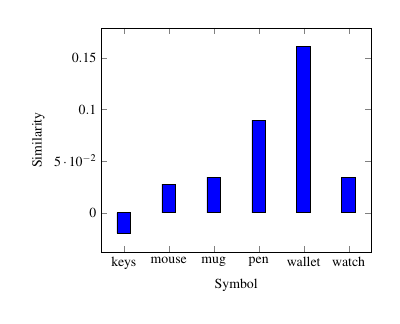
\begin{tikzpicture}[yscale=0.5, xscale=0.5]
        \begin{axis}[
            symbolic x coords={keys, mouse, mug, pen, wallet, watch},
            xlabel = Symbol,
            ylabel = Similarity
          ]
            \addplot[ybar,fill=blue] coordinates {
                (keys,   -0.020032173214673016)
                (mouse, 0.027742071303527464)
                (mug, 0.03443254630997427)
                (pen, 0.089801145874187763)
                (wallet, 0.16100011074269183)
                (watch, 0.034034204029029354)
            };
        \end{axis}
    \end{tikzpicture}	
        \caption{Probe at (-13, 21.5).}
        \label{pgf:bar2}
    \end{subfigure}
    
    			\caption{Similarity test after probing for specific locations}
    \end{figure}

	

		\label{fig:visual-scene-exp}
	
\subsection{Symbolic Scripting (Holographic Controllers)}

We have used our system to create a mechanism for encoding neural programs and processes through a series of associated action, perception and actuator symbols. We call this mechanism for defining controllers using holographic memories "symbolic scripting".


\begin{figure}[th!]
	\center
	\begin{subfigure}{1\columnwidth}
		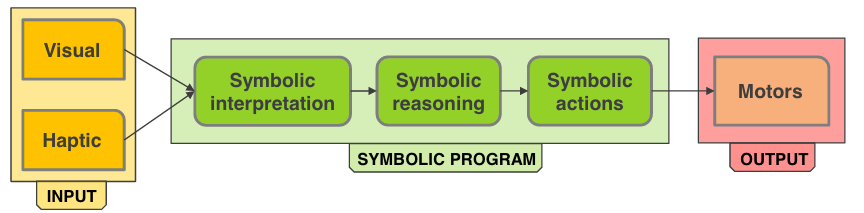
\includegraphics[width=\columnwidth]{img/control_pipeline.png}
		\caption{Symbolic scripting pipeline}
		\label{fig:symbolic-scripting-a}
	\end{subfigure}
	
	
	\begin{subfigure}{0.7\columnwidth}
		\center
		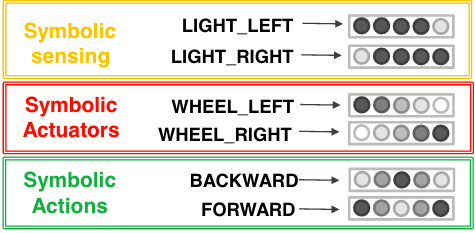
\includegraphics[width=\columnwidth]{img/symbol_table.png}
		\caption{Symbol table}
		\label{fig:symbolic-scripting-b}
	\end{subfigure}
	\begin{subfigure}{1\columnwidth}
		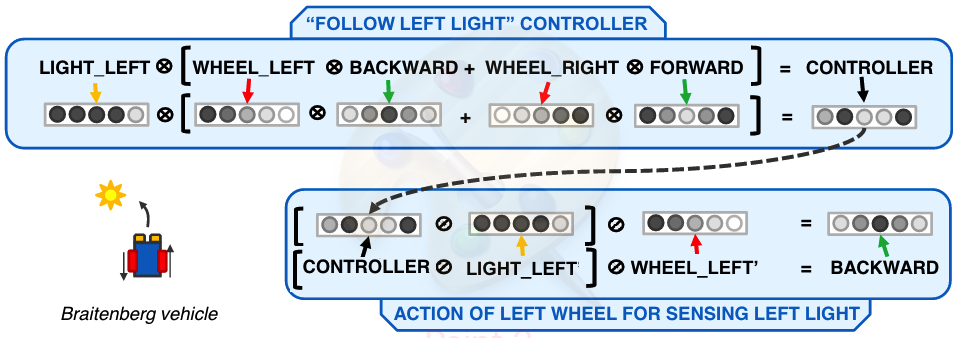
\includegraphics[width=\columnwidth]{img/controller.png}
		\caption{Holographic program (script)}
		\label{fig:symbolic-scripting-c}
	\end{subfigure}
	\caption{Symbolic scripting illustration: object following}
	\label{fig:symbolic-scripting}
\end{figure}


The basic idea is centred around symbolic representations of all three parts involved:
\begin{enumerate}
	\item \textbf{actions} are symbolic constants representing groups of control signals, such as "forward", "backward", "stop", "flex", etc.
	
	\item \textbf{actuators} are named controllable parts of the system on which actions can be performed on, such as "right\_wheel", "left\_wheel", etc.
	
	\item \textbf{senses} are preprocessed (classified) sensory stream labels, such as "bright", "dark", "touching", "falling\_down", "rolling", etc.
\end{enumerate}

An example of this kind of symbolic script is given in figure \ref{fig:symbolic-scripting}. Here the memory encodes an object following behaviour for its left wheel.

		\begin{figure}[th!]
			\begin{subfigure}{0.45\columnwidth}
				\center
				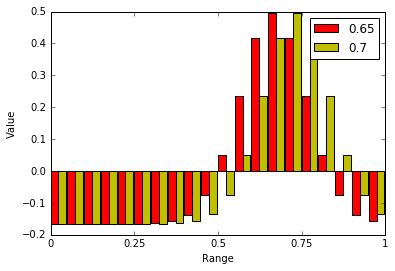
\includegraphics[width=1\columnwidth]{img/gaussianbar.png}
				\caption{Raw input distribution}
				\label{fig:gaussianbar}
			\end{subfigure}
			\begin{subfigure}{0.45\columnwidth}
				\center
				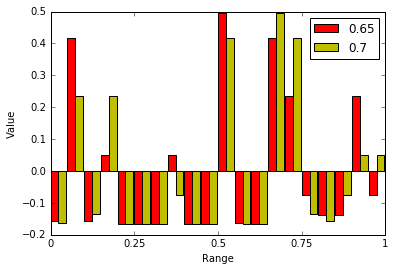
\includegraphics[width=1\columnwidth]{img/gaussianbarperm.png}
				\caption{Permuted distribution}
				\label{fig:gaussianbarperm}
			\end{subfigure}	
		\caption{Sensory input at two successive points in time}
		\label{fig:gaussian}
		\end{figure}	

	In our experiment we have extended the detection of light to a position along the visual field, reduced to the X-axis, rather than just binary statements like "light is visible to the left". To visualize the difference chart \ref{fig:gaussianbar} shows the position of light for two consecutive time steps. The value $0$ represents the far left corner of the sensor, and $1$ the far right one. The chart can be viewed as a (normalized) probability of light being at a certain position, and both cases show it being somewhere right of the center. Chart \ref{fig:gaussianbarperm} shows what the Gaussian distributions look like when they are permuted. This shape of theirs is then used as a symbol. Concretely, instead of encoding a random symbol for "light\_left" we encode a scalar representing the position of light along the visual field and bind it with the rest of the controller components. Accordingly, when running the experiment, once the light reaches a position encoded in the controller it will issue new commands to the vehicle.

The symbolic scripting experiment is set up using a single-sensor Braitenberg
vehicle (see figures \ref{fig:experiment:agent1} and
\ref{fig:experiment:agent2}).
The sensor returns a list of objects in its field of view with their
corresponding view space positions in $[0,1]$ (far left to far right).
% note: it would be better if we probe with all returned objects and check the
% result, but IIRC this did not work well. maybe figure it out?
All returned objects are then compared to the agent's target object.
If the target is found, the holographic controller is probed with its view space
position which, due to the similarity of scalars, yields results even for
values that lie between the originally stored values and can consequently be
probed with the symbols $left\_wheel$ and $right\_wheel$ to extract the symbolic
actions $forwards$ or $backwards$.
If the target is not found or no action could be determined, the agent defaults
to probing the controller with the symbolic constant $no\_object$ which results in
a clockwise rotation when probing for wheel actions (see figure
\ref{fig:experiment:similar2}).

In the left column of figure \ref{fig:experiment}, the agent approaches the blue
target (figure \ref{fig:experiment:agent1}). Following figure {fig:experiment:pos1} in the beginning (tick $-50$), the
agent rotates right (default action) because the target is not visible.
At tick $-30$, the object enters the agent's visual field and continuously nears the fields center, which is reached at tick $-19$.
Then, with the sensory value of ${\sim}0.5$, the actions for both wheels switch
to $forwards$ (figure \ref{fig:experiment:similar1}) and the agent approaches
the target, constantly decreasing its distance
(figure \ref{fig:experiment:distance1}).

In the right column of figure \ref{fig:experiment}, the target is not yet
in the visual field of the agent.
This is the result of the agent previously reaching an old target (at approximately tick $-13$) which lead
to the removal of all current objects and random placement of new ones,
including a new target.
As seen in figure {fig:experiment:pos2} since the new target is placed outside of the agent's field of view, the default
action of probing $no\_object$ is performed. The
clockwise rotation can also be seen in figure \ref{fig:experiment:similar2}). Regardless of how many times the agent reaches its target it will continue to find and pursue new ones solely with the help of its symbolic controller.

This experiment shows the effectiveness of our approach in a practical
application by encoding symbolic sensing, actuators and actions in a
controller.

\begin{figure}%[th!]
\center
\begin{subfigure}{.47\columnwidth}
	\center
	{%
	\setlength{\fboxsep}{0pt}%
	%\setlength{\fboxrule}{1pt}%
	\fbox{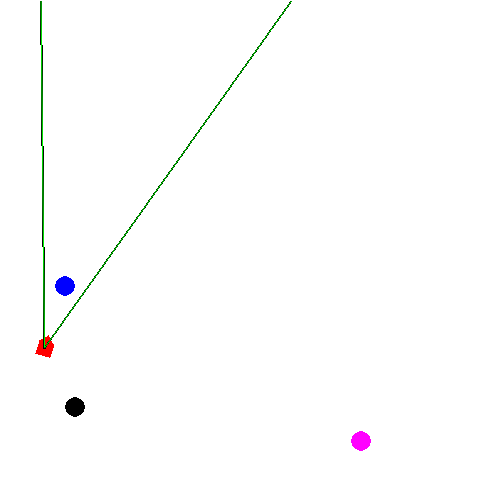
\includegraphics[width=.98\columnwidth]{img/exp_robot_139.png}}%
	}%
	\caption{Blue target visible}
	\label{fig:experiment:agent1}
\end{subfigure}
\begin{subfigure}{.47\columnwidth}
	\center
	{%
	\setlength{\fboxsep}{0pt}%
	%\setlength{\fboxrule}{1pt}%
	\fbox{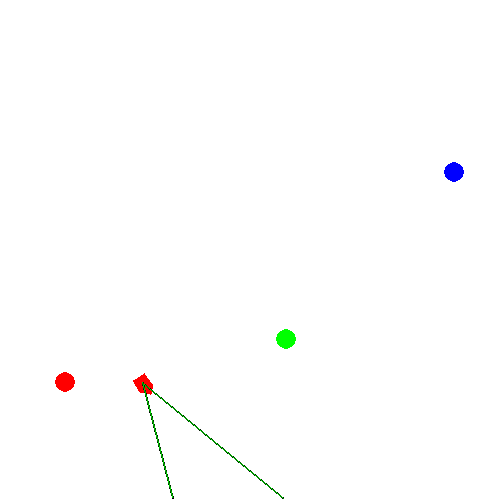
\includegraphics[width=.98\columnwidth]{img/robot_235.png}}%
	}%
	\caption{Blue target not visible}
	\label{fig:experiment:agent2}
\end{subfigure}
\begin{subfigure}{.49\columnwidth}
	\center
	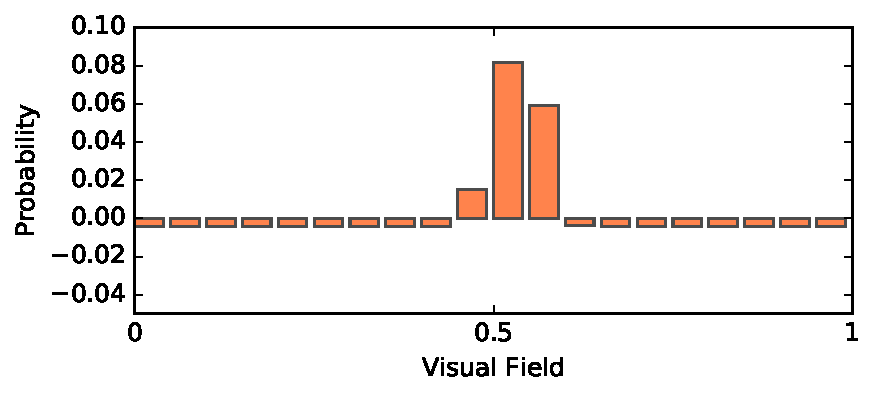
\includegraphics[width=.98\columnwidth]{img/3_139.pdf}
	\caption{Successful sensing}
	\label{fig:experiment:sensor1}
\end{subfigure}
\begin{subfigure}{.49\columnwidth}
	\center
	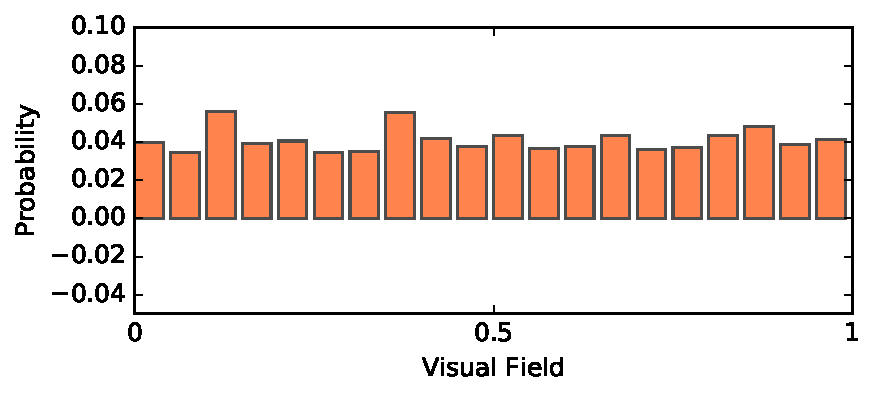
\includegraphics[width=.98\columnwidth]{img/3_235.pdf}
	\caption{Unsuccessful sensing}
	\label{fig:experiment:sensor2}
\end{subfigure}
\begin{subfigure}{.49\columnwidth}
	\center
	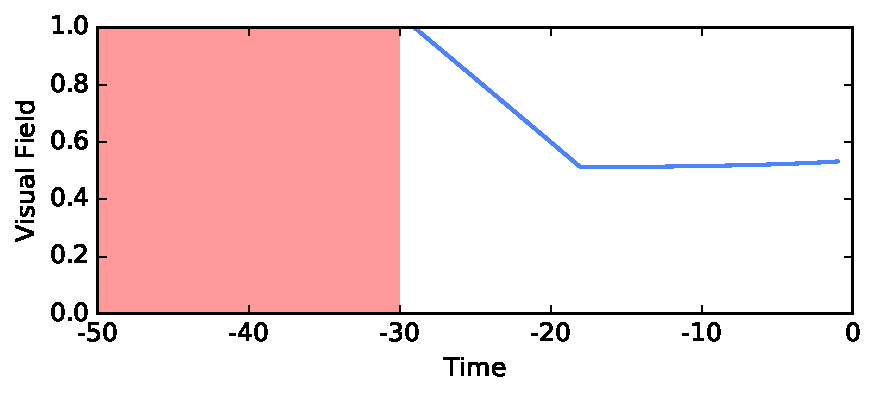
\includegraphics[width=.98\columnwidth]{img/1_139.pdf}
	\caption{Agent 1 run}
	\label{fig:experiment:pos1}
\end{subfigure}
\begin{subfigure}{.49\columnwidth}
	\center
	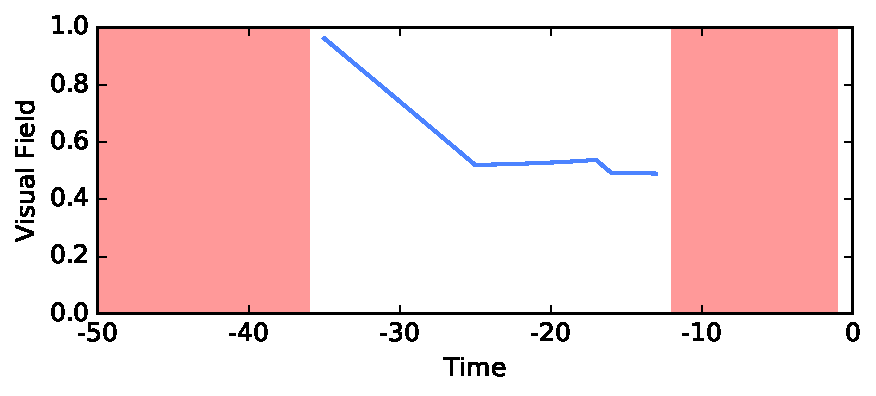
\includegraphics[width=.98\columnwidth]{img/1_235.pdf}
	\caption{Agent 2 run}
	\label{fig:experiment:pos2}
\end{subfigure}
\begin{subfigure}{.49\columnwidth}
	\center
	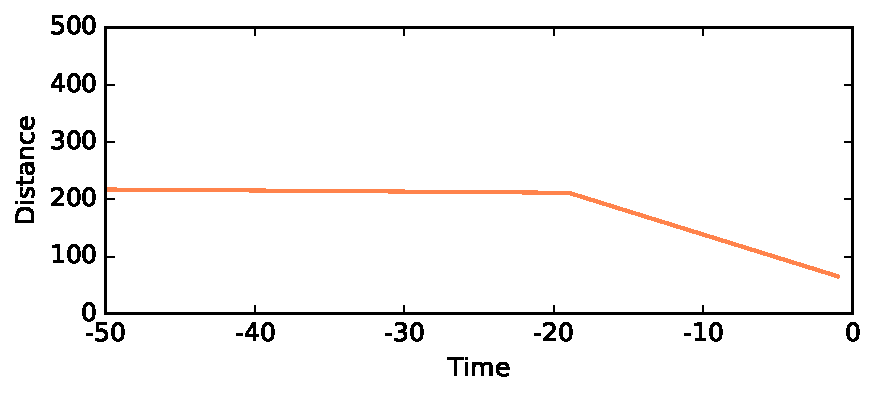
\includegraphics[width=.98\columnwidth]{img/4_139.pdf}
	\caption{Distance Agent 1}
	\label{fig:experiment:distance1}
\end{subfigure}
\begin{subfigure}{.49\columnwidth}
	\center
	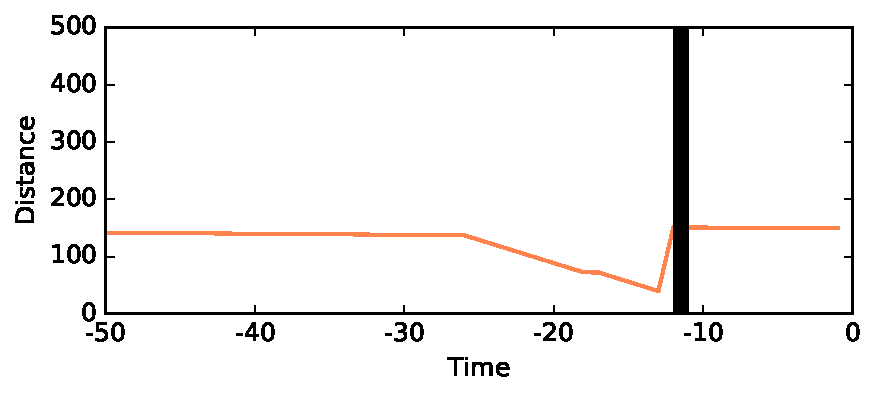
\includegraphics[width=.98\columnwidth]{img/4_235.pdf}
	\caption{Distance Agent 2}
	\label{fig:experiment:distance2}
\end{subfigure}
\begin{subfigure}{.49\columnwidth}
	\center
	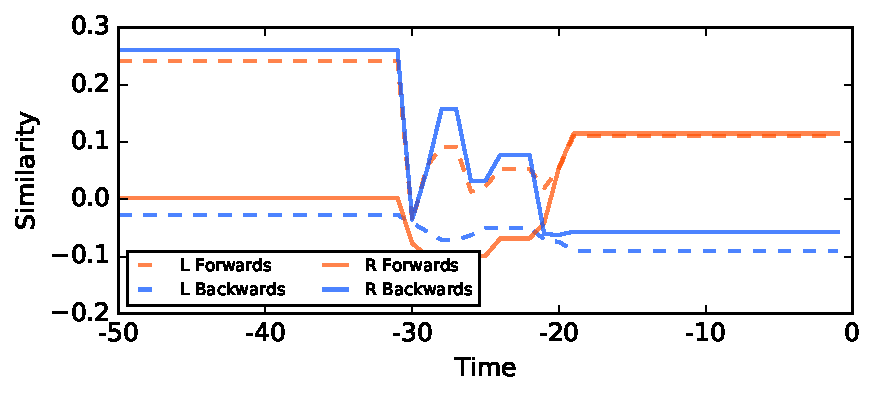
\includegraphics[width=.98\columnwidth]{img/2_139.pdf}
	\caption{Symbol similarity Agent 1}
	\label{fig:experiment:similar1}
\end{subfigure}
\begin{subfigure}{.49\columnwidth}
	\center
	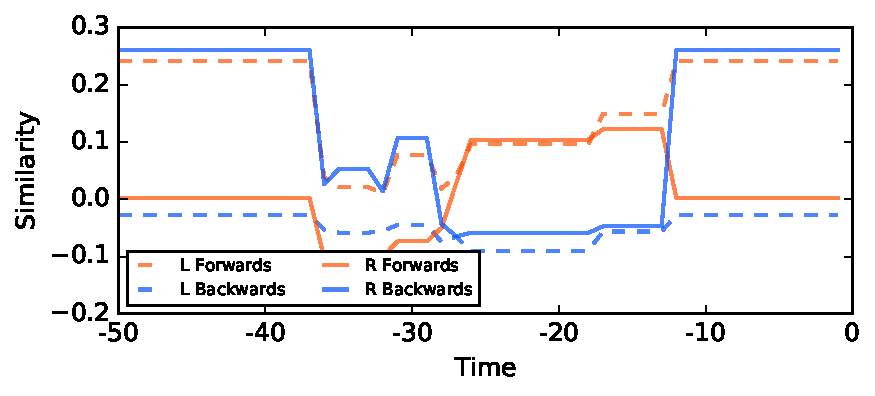
\includegraphics[width=.98\columnwidth]{img/2_235.pdf}
	\caption{Symbol similarity Agent 2}
	\label{fig:experiment:similar2}
\end{subfigure}
\caption{Controlling a vehicle with one linear sensor.}
\label{fig:experiment}
\end{figure}

	\section{CONCLUSIONS}
	We have introduced a mechanism for intrinsic symbol encoding/decoding for Holographic Reduced Representations.
As a consequence, our approach eliminates the need for clean-up memories as they are described in literature.
Instead, results of probing operations directly give interpretable symbols, which can be decoded in constant computational time.
In other words, time needed for encoding/decoding is completely independent of the total number of symbols memorized.\\
	A concrete biophysical evidence and theoretical model of implementation of convolution in the brain is, unfortunately, still missing. Nevertheless, our work assumes convolution as the basic computational substrate of higher level cognition and identifies random permutation as computational requirement without which association of probabilistically encoded symbols is not possible.
	
	
\vfill
\bibliographystyle{apalike}
{\small
\bibliography{example}}


%\section*{\uppercase{Appendix}}
%
%\noindent If any, the appendix should appear directly after the
%references without numbering, and not on a new page. To do so please use the following command:
%\textit{$\backslash$section*\{APPENDIX\}}

\vfill
\end{document}

